\documentclass[12pt]{article}
\usepackage{amssymb,amsmath,graphicx,mathtools}
\usepackage{listings}
\usepackage[margin=0.75in]{geometry}
\parindent 16 pt
\usepackage{fancyhdr}
\pagestyle{fancy}
\fancyhead[R]{Swupnil Sahai}
\fancyhead[C]{04/05/16}
\fancyhead[L]{Kernel Model}
\DeclarePairedDelimiter\ceil{\lceil}{\rceil}
\DeclarePairedDelimiter\floor{\lfloor}{\rfloor}

\lstset{
    language=R,
    basicstyle=\scriptsize\ttfamily,
    stepnumber=1,
    numbersep=5pt,
    showspaces=false,
    showstringspaces=false,
    showtabs=false,
    frame=single,
    tabsize=2,
    captionpos=b,
    breaklines=true,
    breakatwhitespace=false,
    escapeinside={},
    keywordstyle={},
    morekeywords={}
    }

\begin{document}

% CUSTOM SHORTCUTS

\def\ci{\perp\!\!\!\perp}
\def\ex{\mathbb{E}}
\def\prob{\mathbb{P}}
\def\ind{\mathbb{I}}
\def\grad{\triangledown}
\def\bigo{\mathcal{O}}

%MODEL FORUMLATION
\subsection*{Motivation}
The original kernel model assumed that the distribution of ages for each name could be well approximated by a normal distribution. Since we found that the assumption does not hold, it is better to just use the discrete empirical distribution.

\subsection*{Formulation}
The negative binomial expression is the same as before:

$$ y_{ik} \sim \text{NegBin}(\omega_k \mu_{ik}, \omega_k)
\hspace{20 pt} E(y_{ik}) = \mu_{ik} 
\hspace{20 pt} Var(y_{ik}) = \mu_{ik} + \frac{\mu_{ik}}{\omega_k}$$

\noindent  Now let $a_i \in \{0,\dots,100\}$ and $g_i \in \{M,F\}$ denote the age and gender of ego $i$, respectively, while we let $g_k$ denotes the gender of alter name $k$. Then we can derive the mean expression as follows:

$$ \mu_{ik} = N_i p(k|a_i,g_i)
= N_i \sum_{s=2}^{100} p(k|s,g_k) p(s,g_k|a_i,g_i) 
= N_i \sum_{s=2}^{100} p(k|s,g_k) p(s|a_i) p(g_k|g_i)$$
$$ = N_i  p(g_k|g_i) \sum_{s=2}^{100} p(k|s,g_k) p(s|a_i)
= N_i p_{g_ig_k}  \sum_{s=2}^{100} \frac{p(k,s,g_k)}{p(s,g_k)} \frac{1}{C_{g_ig_k}} \mathcal{K}_{g_ig_k}(a_i,s)$$
$$ = \frac{N_i p_{g_ig_k}}{C_{g_ig_k}} \sum_{s=2}^{100} \frac{p(k,s,g_k)}{p(s,g_k)} \mathcal{K}_{g_ig_k}(a_i,s)$$

\noindent The kernel is defined similar to before but with a discrete normalizing constant:

$$ \mathcal{K}_{g_ig_k}(a_i, a_k) = e^{-\frac{(a_i-a_k)^2}{2\lambda_{g_ig_k}}} 
\hspace{20 pt}
C_{g_ig_k} = \sum_{s=2}^{100}  \mathcal{K}_{g_ig_k}(a_i, s) $$

\vspace{15 pt} \noindent We thus need to estimate $p_{g_ig_k}$ (2 values), $\lambda_{g_ig_k}$ (4 values), $N_i$ (N values), and $\omega_k$ (K values).

%SIMULATION%
\subsection*{Simulation}
We simulate responses to questions about 12 names using estimated age means/variances (for each name) and simulated respondent degrees, name overdispersions, and kernel lambdas in an attempt to see whether our model can recover the correct degrees, overdispersions, and lambdas:

$$\log N_i \sim \mathcal{N}(6.2,0.5) \hspace{20 pt}  \frac{1}{ \frac{1}{\omega_k}+1} \sim Beta(10,2) 
$$

\noindent \begin{tabular}{c | cccccccccccc} 
$k$ & Linda & Jen. & Karen & Kim. & Emily & Steph. & Mark & Jacob & Kevin & Kyle & Adam & Bruce \\
\hline
$\omega_k$ & 5.13 & 19.2 & 2.44 & 16.5 & 2.36 & 5.78 & 3.93 & 20.7 & 14.1 & 4.56 & 5.97 & 7.38  \\
\end{tabular}\\

$$ \lambda
= \left( \begin{array}{cc} \lambda_{FF} & \lambda_{FM} \\
\lambda_{MF} & \lambda_{MM} \end{array} \right) 
= \left( \begin{array}{cc}
225 & 100 \\
144 & 256 \end{array} \right) 
\hspace{20 pt} M
= \left( \begin{array}{cc} p_{FF} & p_{FM} \\
p_{MF} & p_{MM} \end{array} \right) 
= \left( \begin{array}{cc}
0.6 & 0.4 \\
0.45 & 0.55 \end{array} \right)$$

%RESULTS%
\subsection*{Results}
The model does a decent job of recovering the gender mixing probabilities:
$$ M_{BAYES}
= \left( \begin{array}{cc}
0.587 & 0.413 \\
0.435 & 0.565 \end{array} \right) $$

\noindent The model does a terrible job of recovering the lambdas, the with values off by a factor of 1000.

$$ \lambda_{BAYES}
= \left( \begin{array}{cc}
16019 & 9651 \\
14805 & 1129 \end{array} \right) $$

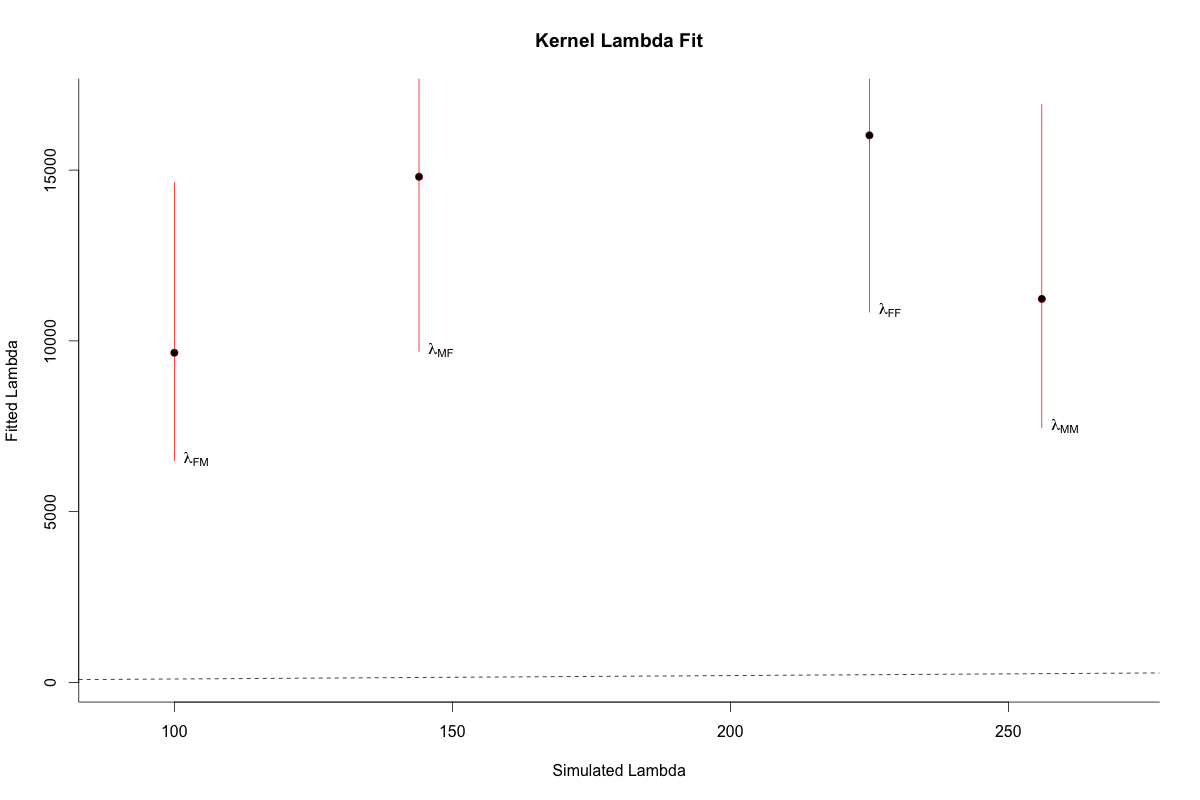
\includegraphics[scale = 0.39]{Lambda_Estimates.png}

\pagebreak
\noindent The degrees are not recovered very well either, with a correlation of only 0.68 between the simulated values and their posterior means.

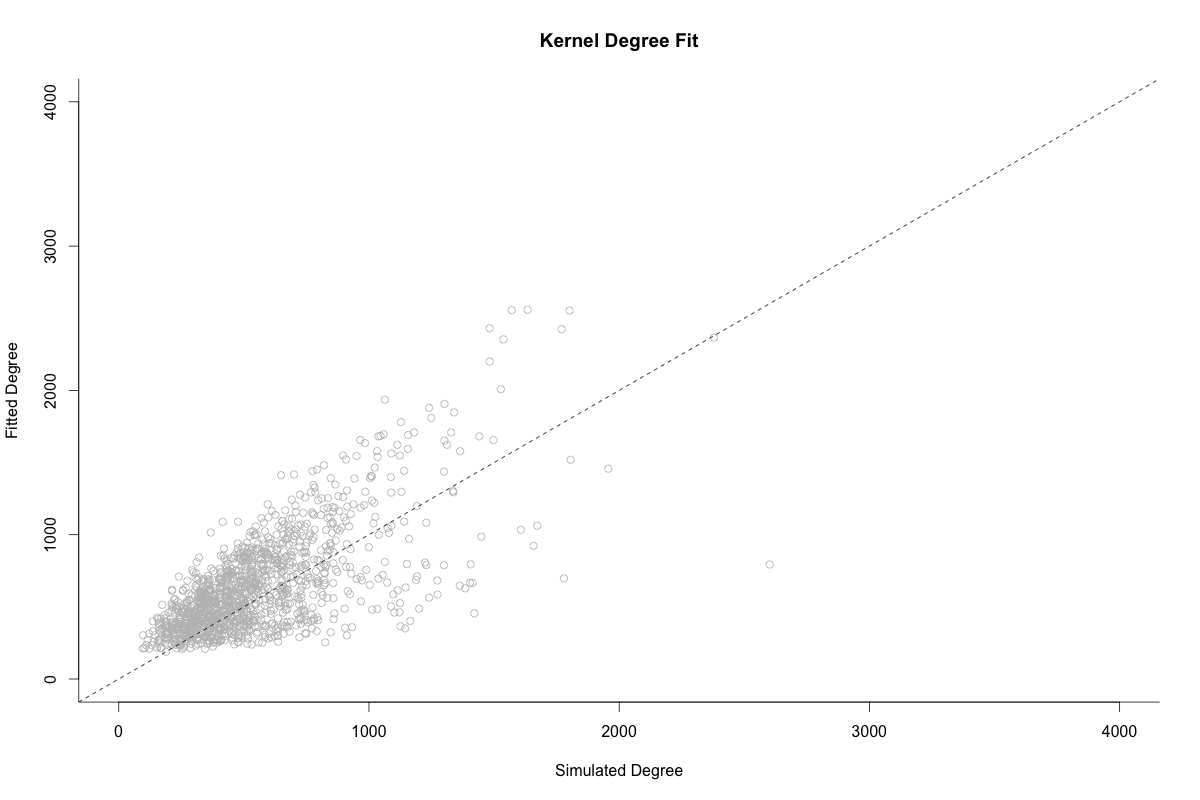
\includegraphics[scale = 0.38]{Degree_Estimates.png}

\noindent None of the overdispersions are contained within the central 95\% of their posterior distributions.

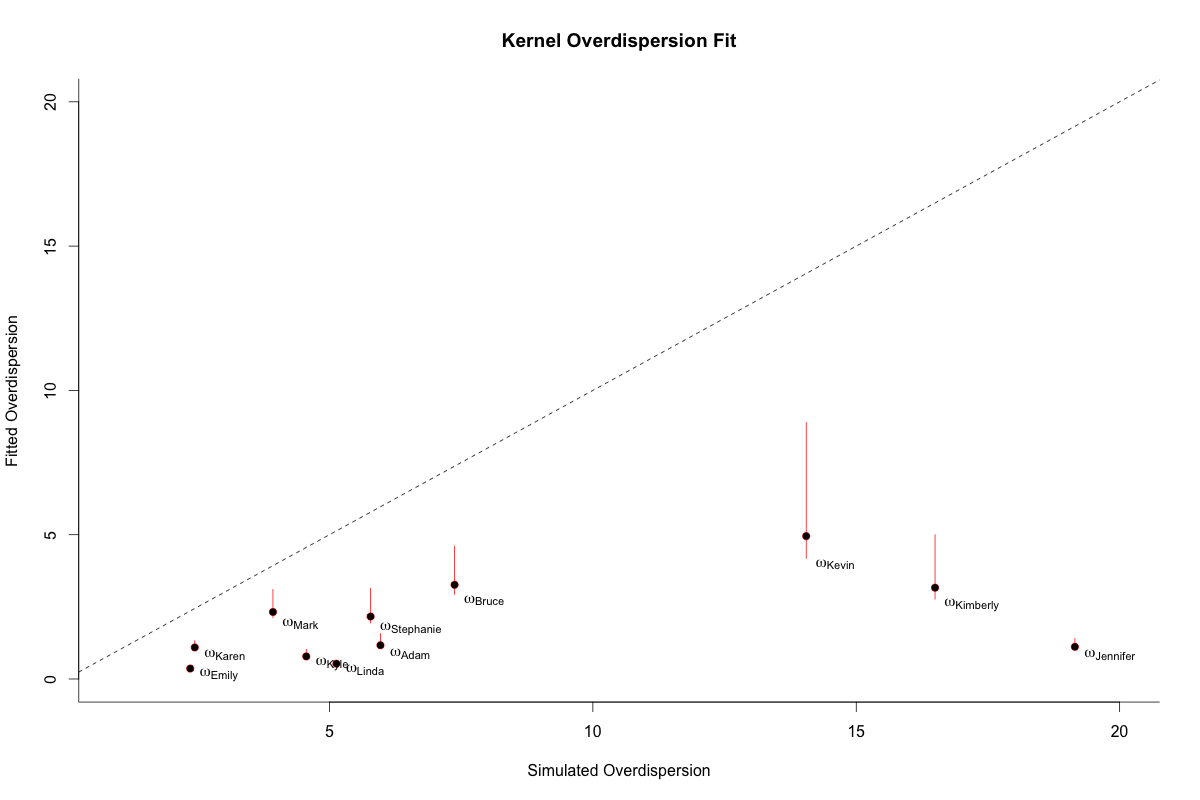
\includegraphics[scale = 0.38]{Overdispersion_Estimates.png}

\end{document}